\begin{table}[]
\centering
\caption{Результаты измерений скорости счета от расстояния до источника в счетчике Гейгера}
\label{t_data_final}
\begin{tabular}{|c|c|c|c|}
\hline
\rowcolor[HTML]{C6E0B4} 
l, мм & t, c & N & $\sigma_N$ \\ \hline
10,00 & 20,1 & 333 & 18 \\ \hline
15,00 & 20,2 & 290 & 17 \\ \hline
16,00 & 19,7 & 255 & 16 \\ \hline
16,50 & 20,6 & 217 & 15 \\ \hline
17,00 & 19,9 & 160 & 13 \\ \hline
17,50 & 19,8 & 98 & 10 \\ \hline
17,75 & 41,7 & 99 & 10 \\ \hline
18,00 & 101,3 & 105 & 10 \\ \hline
18,25 & 99,9 & 83 & 9 \\ \hline
18,50 & 100,4 & 59 & 8 \\ \hline
18,75 & 100,3 & 57 & 8 \\ \hline
19,00 & 105,3 & 73 & 9 \\ \hline
20,00 & 111,8 & 55 & 7 \\ \hline
21,00 & 100,2 & 27 & 5 \\ \hline
\end{tabular}%
\end{table} 

\begin{figure}[H]
    \centering
    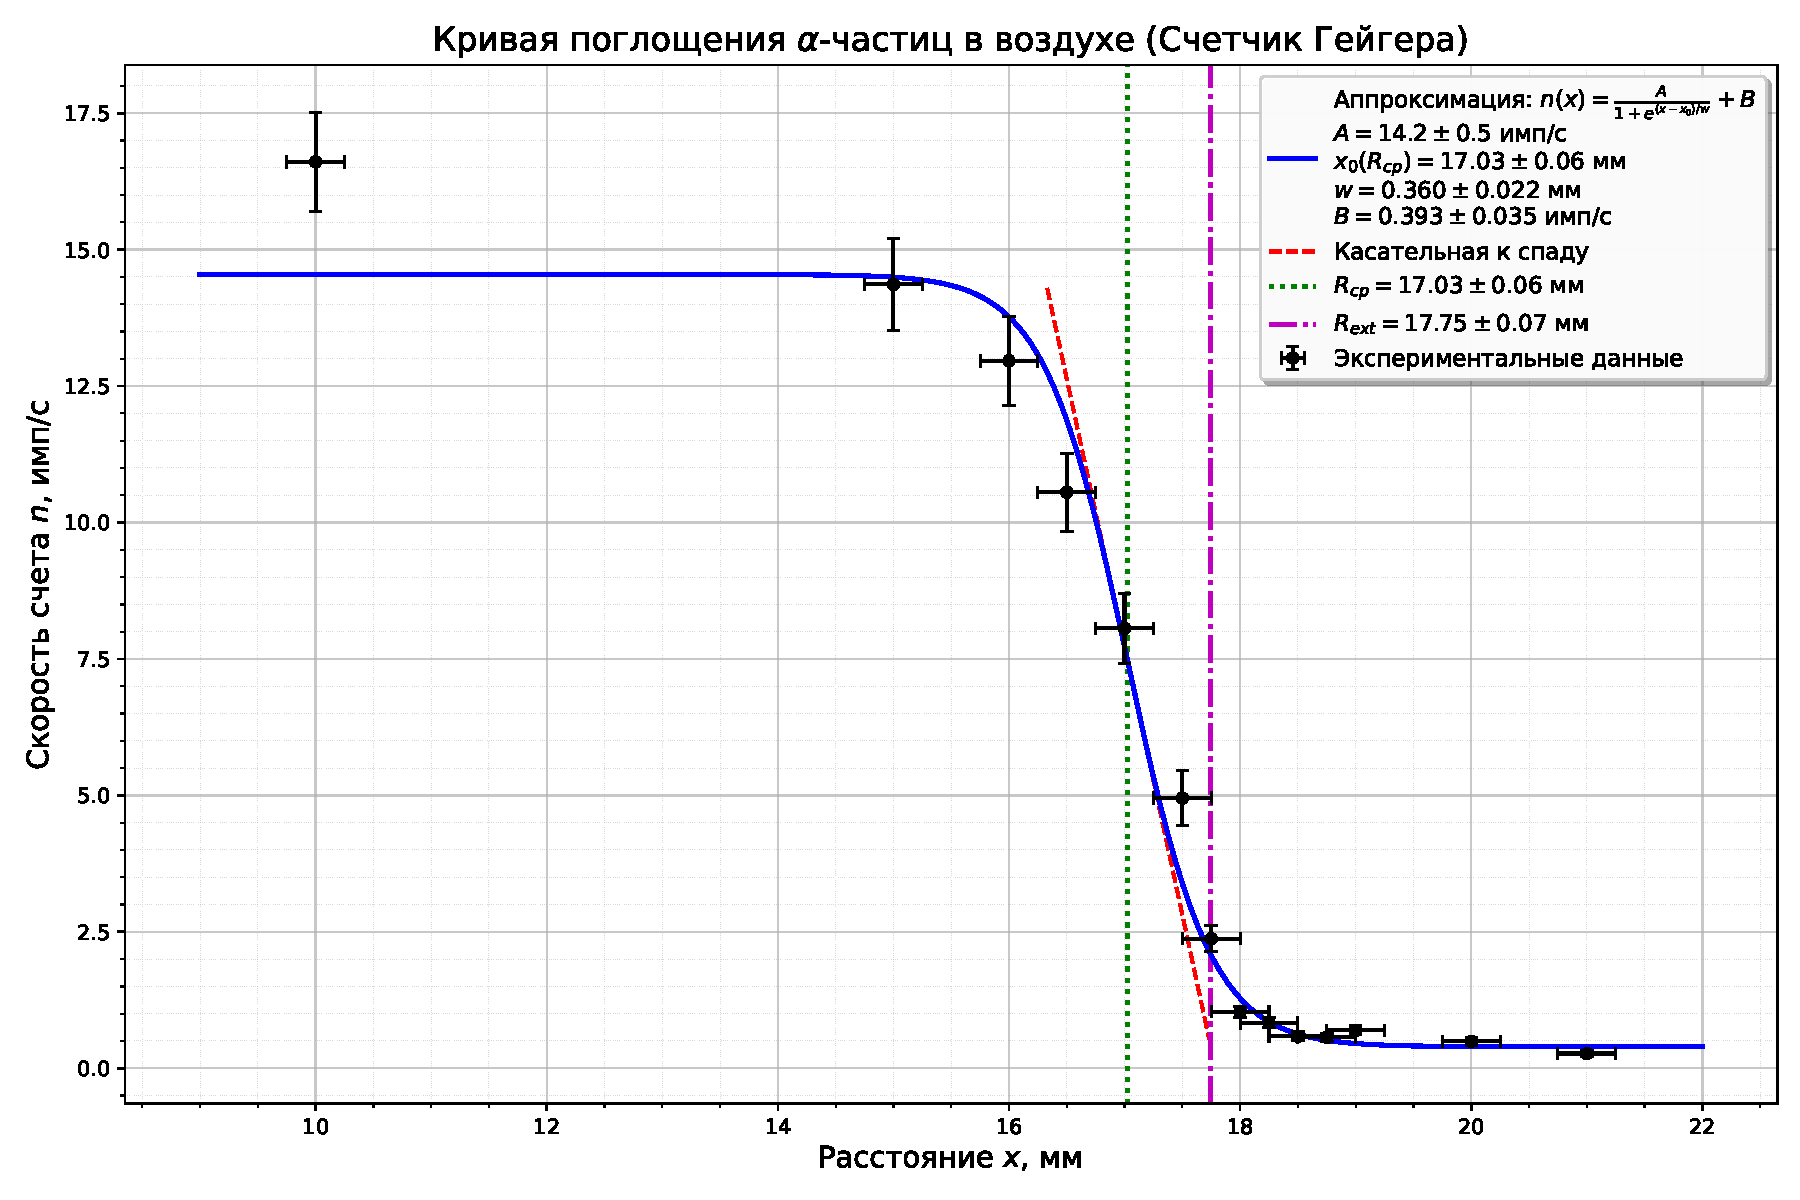
\includegraphics[width=1\textwidth]{pictures/plot_pogl.pdf} % Замените "example-image" на имя вашего файла изображения
    \caption{}
    \label{}
\end{figure}

\begin{table}[]
\centering
\caption{Данные измерений скорости счета в зависимости от давления в осцилляционном счетчике}
\label{t_data}
\begin{tabular}{|c|c|c|}
\hline
\rowcolor[HTML]{C6E0B4} 
P, Торр & t, с & N \\ \hline
13 & 10 & 2892 \\ \hline
33 & 10 & 2610 \\ \hline
53 & 10 & 2236 \\ \hline
73 & 10 & 1812 \\ \hline
93 & 10 & 1468 \\ \hline
113 & 10 & 1099 \\ \hline
133 & 10 & 812 \\ \hline
153 & 10 & 529 \\ \hline
173 & 10 & 352 \\ \hline
193 & 10 & 229 \\ \hline
213 & 10 & 134 \\ \hline
233 & 10 & 86 \\ \hline
253 & 10 & 76 \\ \hline
303 & 10 & 7 \\ \hline
353 & 10 & 5 \\ \hline
353 & 100 & 20 \\ \hline
753 & 200 & 34 \\ \hline
\end{tabular}%
\end{table}

\begin{figure}[H]
    \centering
    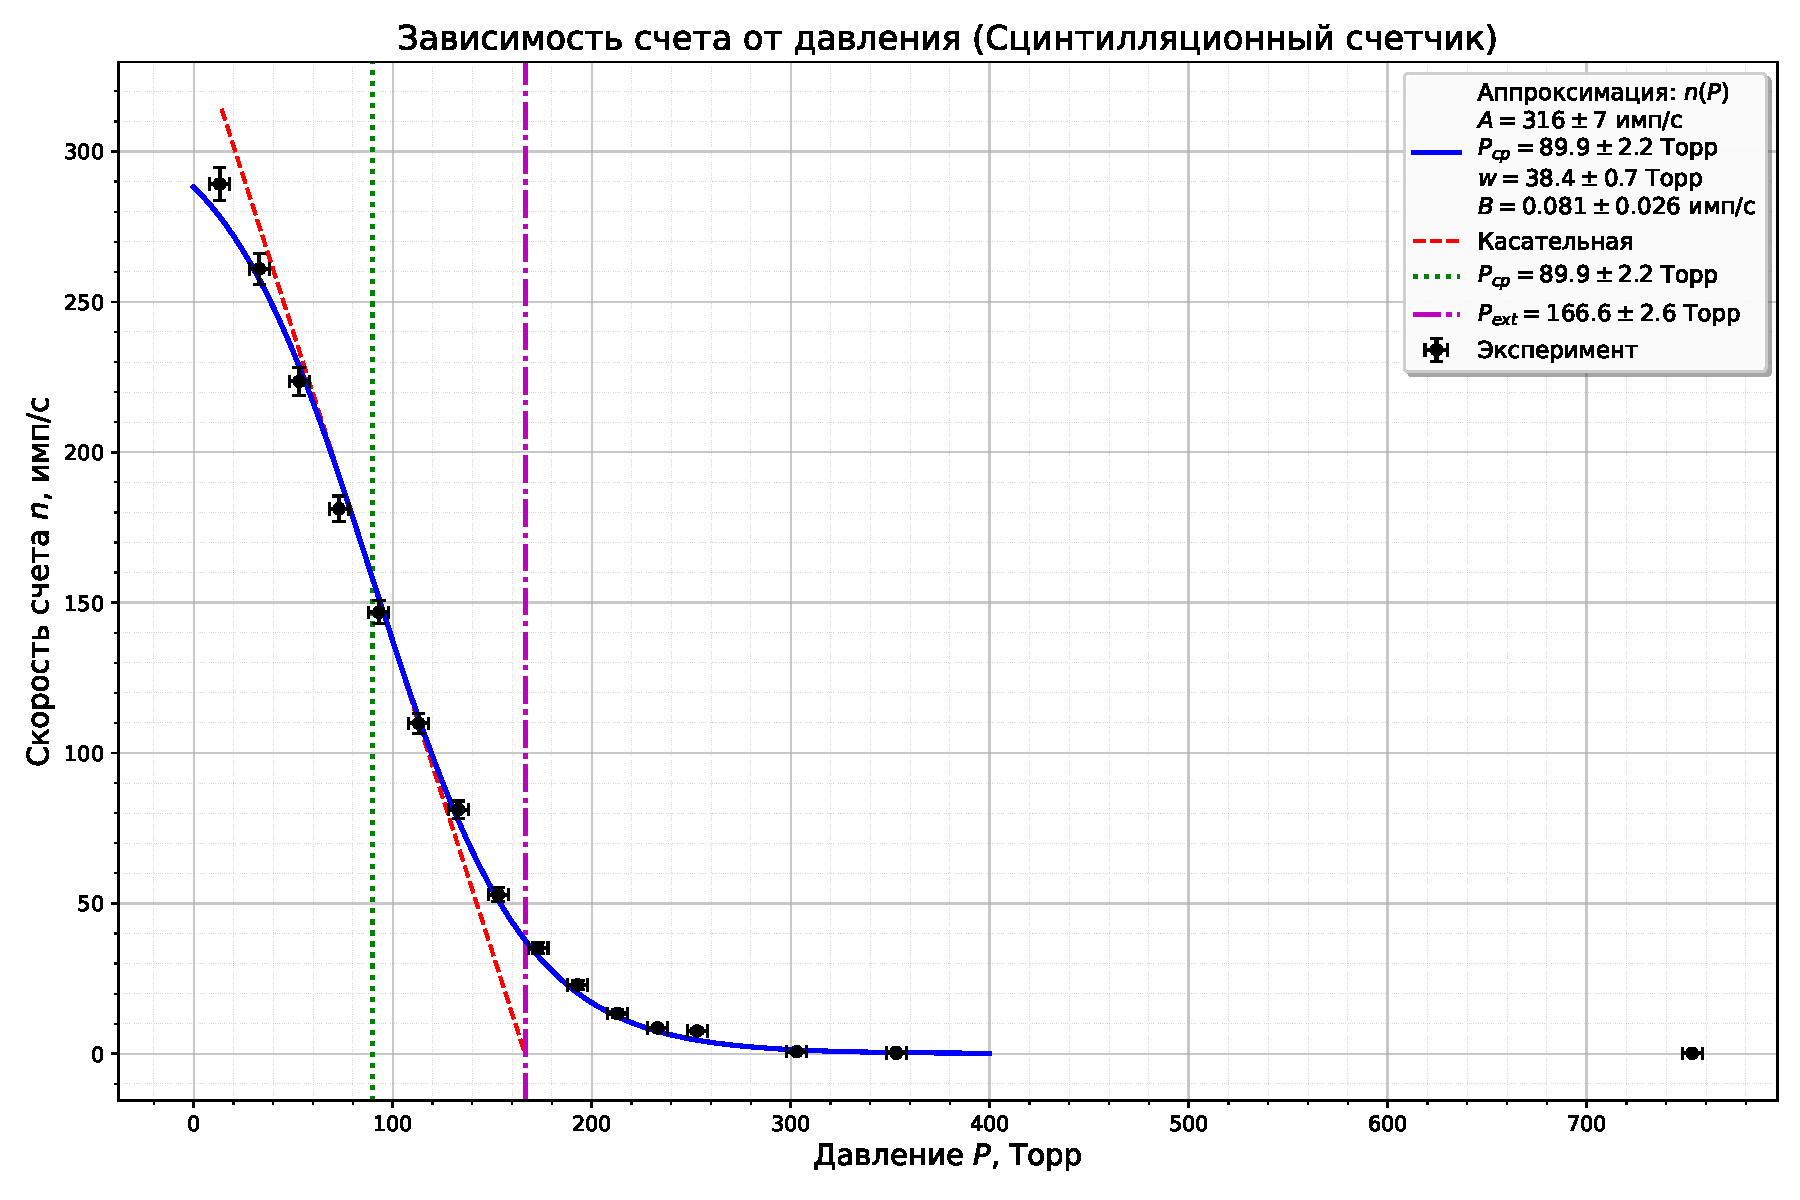
\includegraphics[width=1\textwidth]{pictures/plot2.pdf} % Замените "example-image" на имя вашего файла изображения
    \caption{}
    \label{}
\end{figure}

\begin{table}[]
\centering
\caption{Зависимость тока от давления в ионизационной камере}
\label{t4}
\begin{tabular}{|c|c|}
\hline
\rowcolor[HTML]{C6E0B4} 
P, Торр & I, pA \\ \hline
13 & 5 \\ \hline
63 & 74 \\ \hline
108 & 132 \\ \hline
153 & 196 \\ \hline
203 & 267 \\ \hline
253 & 349 \\ \hline
303 & 427 \\ \hline
353 & 513 \\ \hline
403 & 600 \\ \hline
453 & 676 \\ \hline
498 & 750 \\ \hline
553 & 790 \\ \hline
593 & 790 \\ \hline
653 & 780 \\ \hline
703 & 770 \\ \hline
753 & 753 \\ \hline
\end{tabular}%
\end{table}

\begin{figure}[H]
    \centering
    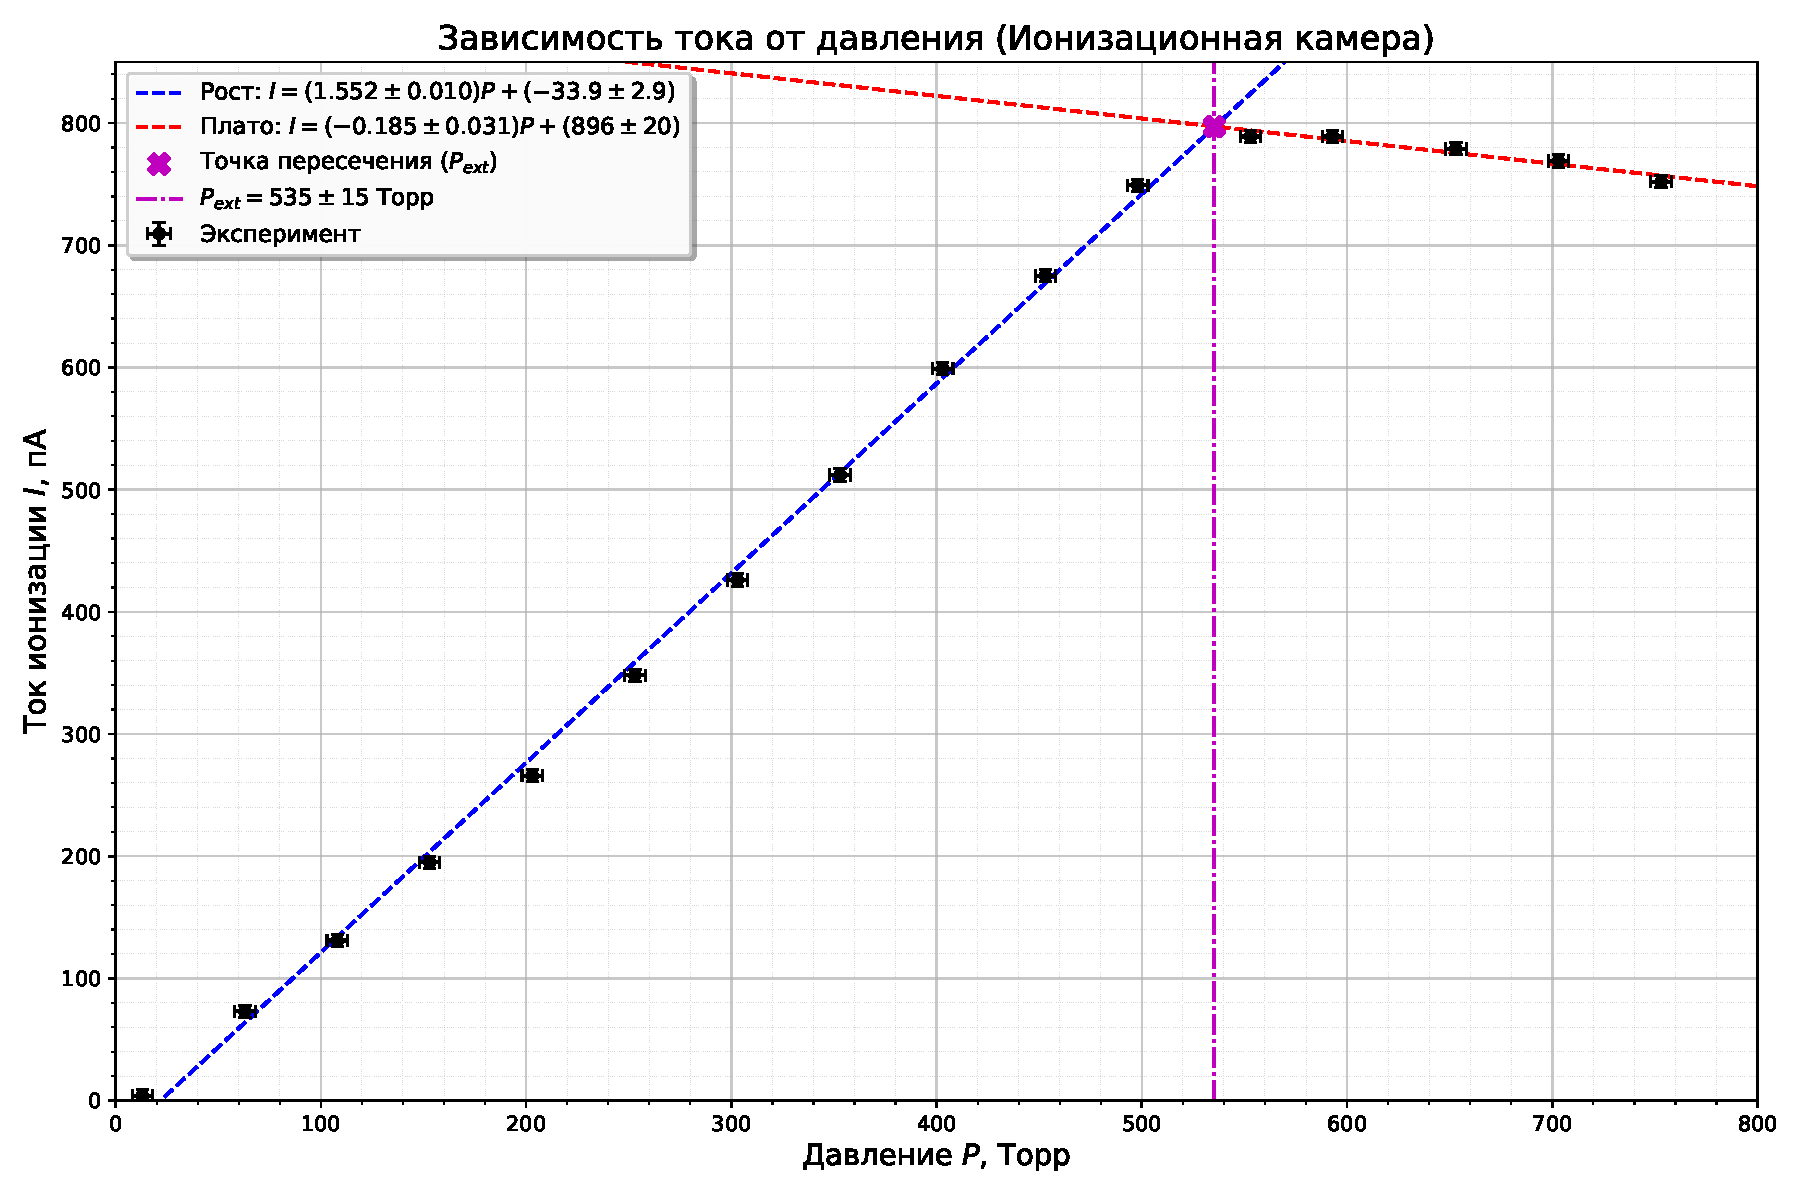
\includegraphics[width=1\textwidth]{pictures/plot3.pdf} % Замените "example-image" на имя вашего файла изображения
    \caption{}
    \label{}
\end{figure}